\section{Related works}

% Introduction

\subsection{Phong Vũ}
\begin{figure}[H]
    \centering
    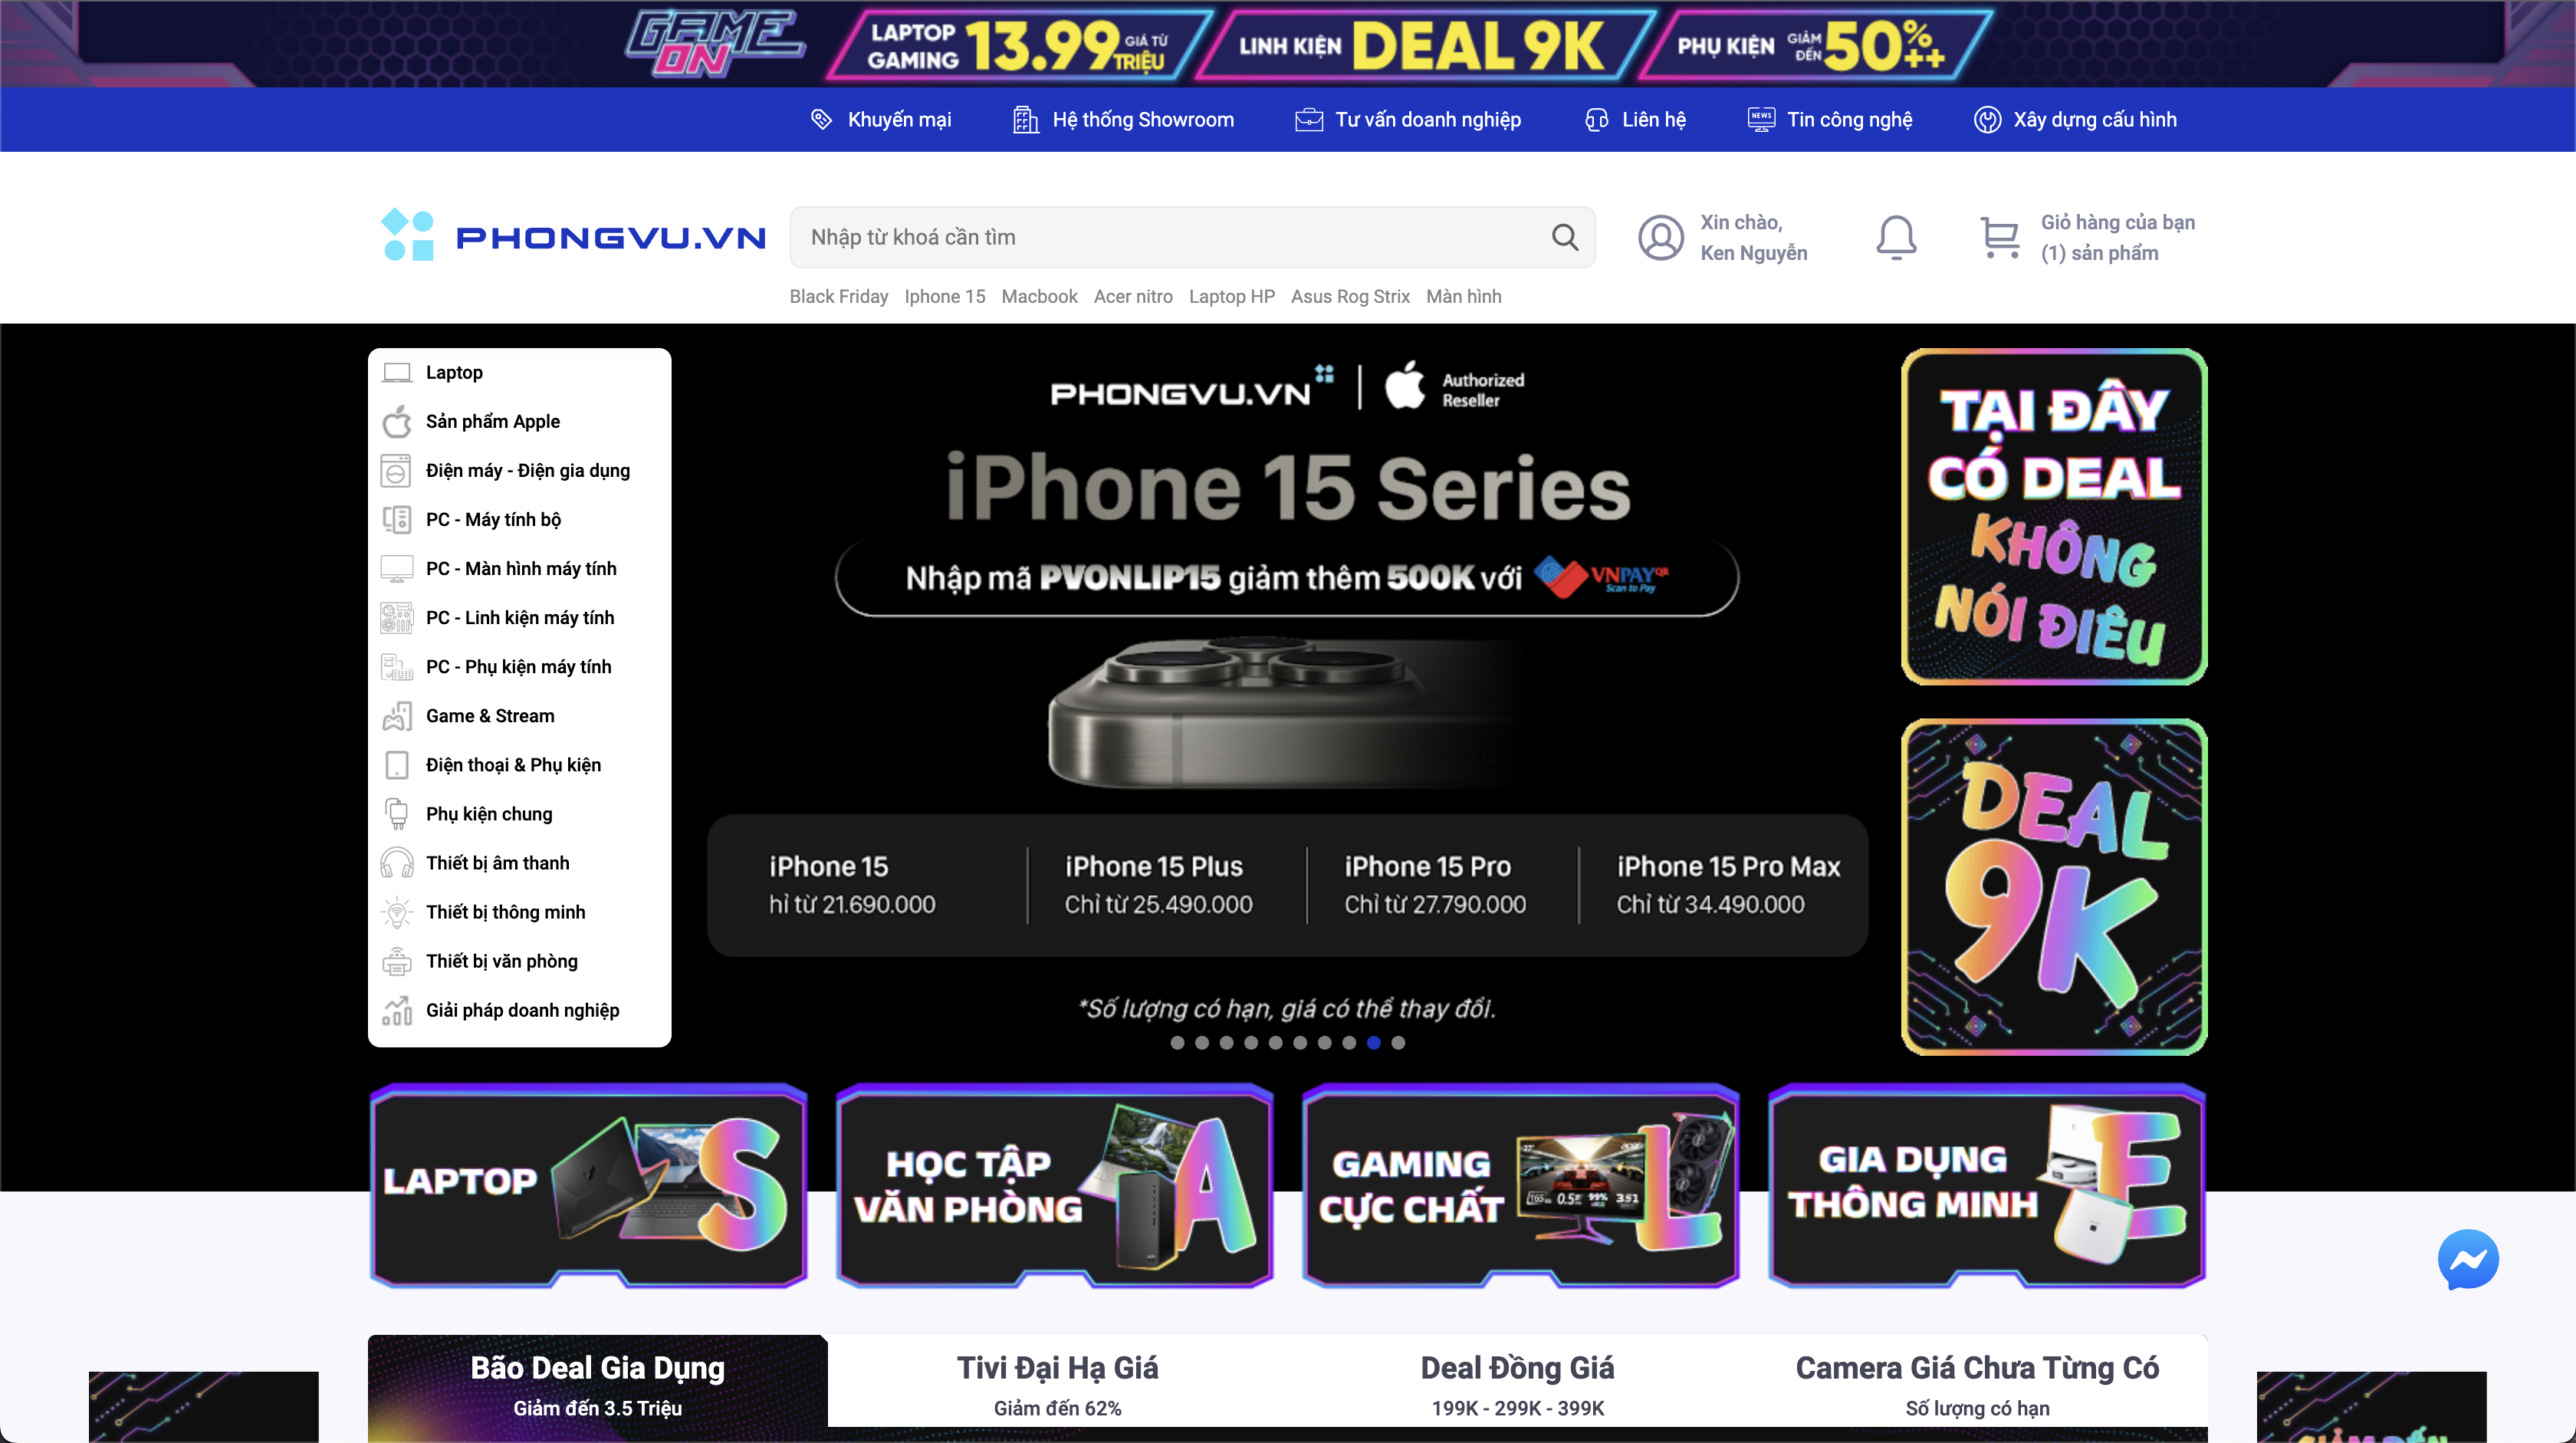
\includegraphics[width=1\linewidth]{image/related-works/phongvu.png}
    \caption{Phong Vũ}
    \label{fig:phong_vu}
\end{figure}

\noindent When mentioning electronics and tech-related retailer in Vietnam, Phong Vu shows it domination in this industry with 35 branches and showrooms across the country. This chain store system has been popular for many years and has gained trust from customers by selling products that meet their growing needs. Potential customers can find all of the electronic devices or technology items here, such as laptops, smartphones, gaming gears, or even office devices. To match the consolidation itself, Phong Vu's website delivers an eye-catching user interface and satisfied experience with some significant features, including:
\begin{itemize}
    \item A structured categories-based products system
    \item Recommendation system with personalized content
    \item Customer-centric PC building page
    \item Entrepreneur consulting services
    \item Technology blogs
\end{itemize}

\noindent From our observation, Phong Vũ computer has done a great job in matching customers demands by supplying massive ranges of products and providing a PC building page. However, it lacks users reviewing section that can reflect real product quality which plays an important role in a retailer application. Moreover, technology blogs feature may seem a little bit off-tracking from a customer glance.

\subsection{MDComputers}

\begin{figure}[H]
    \centering
    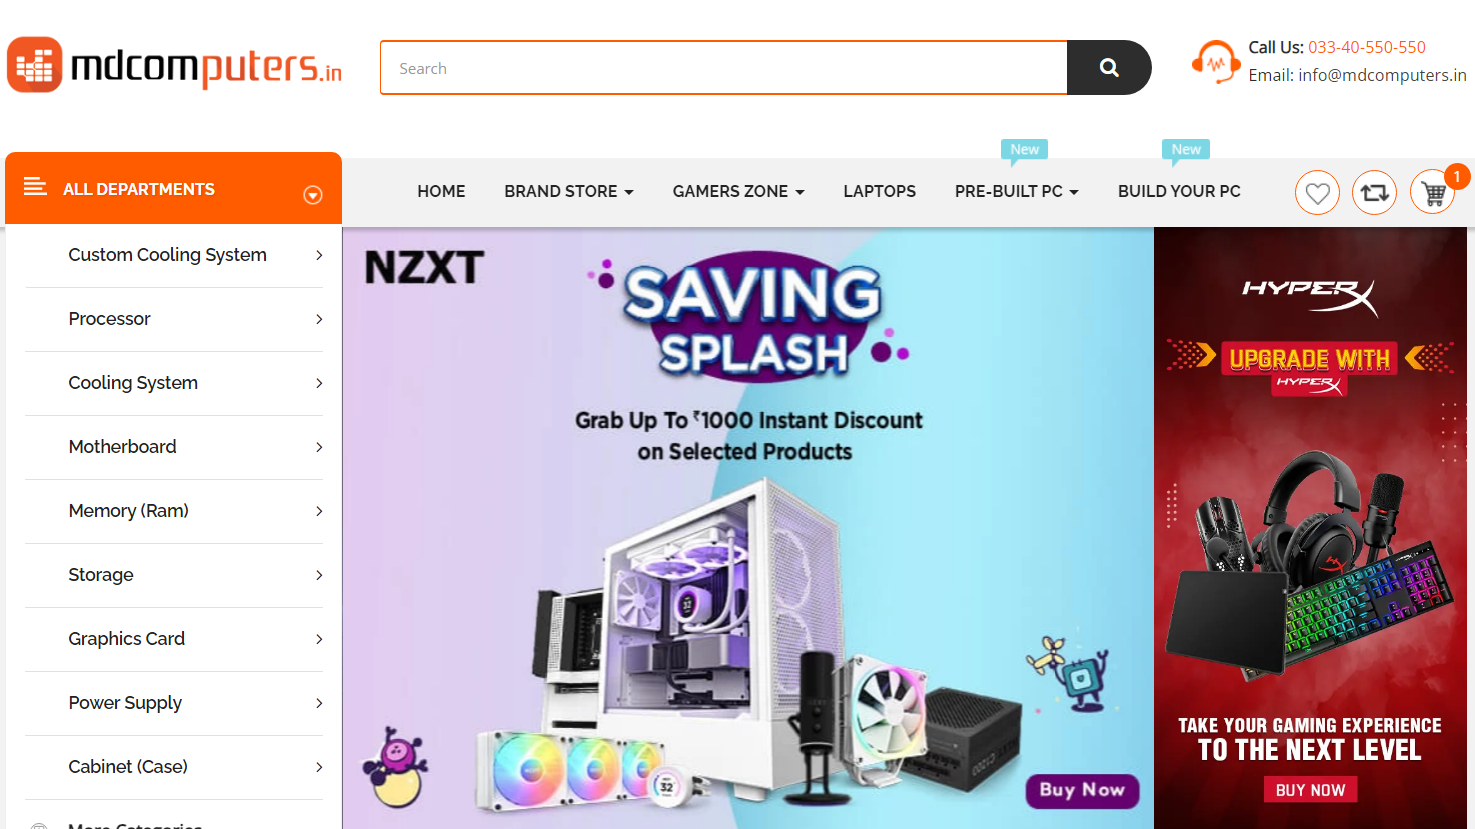
\includegraphics[width=1\linewidth]{image/related-works/mdcomputer.PNG}
    \caption{MDComputers}
    \label{fig:mdcomputer}
\end{figure}

\noindent MDComputer is an old, established electronic equipment website that has been in operation for more than 10 years, with many products of different brands and codes for both PC and laptop users. MDComputer's website supports users with the following features:
\begin{itemize}
    \item Comparing devices: MDComputer has a function to help users view comparison tables of similar products most intuitively, users do not need to remember every detail of the product.
    \item Loyalty points: MDComputer has a reward points system for all customers who have purchased any of their products, increasing the possibility of users to return to the store.
    \item Building PC: Shop has function for users to customize according to individual needs of each customer.
    \item User review and Q\&A: increase the credibility and reliability of the website, provide the practicality of the products to potential customers.
\end{itemize}
In addition to the basic functions of an e-commerce website, MDComputer has functions that provide customers with more experiences and new choices on a diverse product platform. The store's contact options are limited to email and direct phone calls. Unfortunately, there is no chat feature available for users who may prefer or require instant messaging assistance but MDComputer still excels in other areas, making their platform worth learning from and referencing